\chapter[Metodologia]{Metodologia}

Essa seção é dividida em dois grandes blocos, que elucidam duas grandes etapas do projeto. Primeiramente, tem-se a prova de conceito, no qual fluxogramas visam explanar a lógica de funcionamento, apontando qual é a entrada e a saída daquele bloco, bem como, qual é o processamento realizado. A prova de conceito foi implementada em um \textit{software} de síntese musical chamado \textit{PureData}.


Em seguida, encontra-se a seção da implementação final realizada. Essa seção é divivida em duas subseções: uma dedicada ao \textit{hardware}, que explica como os sinais de controle foram obtidos e como o sinal de saída se dá para que possa ser reproduzido em um sistema de som, e outra dedicada ao \textit{software}, que engloba a aquisição do sinal através de arquivos de música no formato \textit{.wav}, explicações de aquisição de sinais analógicos convertidos para digitais, que são responsáveis pelos controles de frequência, escolha do efeito e a quantidade de efeito aplicado, além do processo de construção do filtro utilizado na aplicação.

\section{Proposta Geral}

A evolução dos equipamentos de mixagem começou com a mixagem em vinil, e ao longo do tempo, novas funcionalidades foram adicionadas, como o \textit{jogger} para atraso e avanço da música, \textit{fader} para controle de volume e \textit{knobs} para ajuste de frequências. Com o avanço da microeletrônica, esses equipamentos evoluíram para a eletrônica digital, incorporando \textit{DSPs} para processar formatos de áudio de alta qualidade, como WAV e FLAC.

Atualmente, existem dois tipos principais de equipamentos de mixagem: os mais caros, que não requerem um computador, e os mais acessíveis, que dependem de um computador, mas oferecem melhor qualidade de processamento. DJs iniciantes frequentemente enfrentam dificuldades para realizar ajustes finos nas bandas de frequência em \textit{mixers} clássicos de três bandas. Esta habilidade é crucial para destacar elementos musicais e criar novas atmosferas. À medida que um DJ desenvolve seu estilo, a mixagem torna-se mais automática, facilitando a transição entre músicas.

Este projeto propõe a criação de um \textit{mixer} com um controle central que manipula dois arquivos de música. Em vez dos tradicionais controles de três bandas de frequência, o \textit{mixer} utilizará filtros passa-altas. O controle central ajustará simultaneamente as frequências de corte de ambos os canais, permitindo uma transição suave entre as músicas.

Além disso, o sistema incluirá dois efeitos, \textit{delay} e \textit{reverb}, que serão controlados através de um botão giratório, que determinará a intensidade do efeito aplicado.

Em resumo, o sistema processará arquivos de áudio que já estejam dentro da \textit{Raspberry Pi}, utilizando filtros passa-altas e permitindo ao usuário selecionar e controlar a intensidade dos efeitos, com botões \textit{knobs} para ajuste e um botão \textit{on}/\textit{off} para seleção dos efeitos.

\section{Levantamento de Requisitos}

O levantamento de requisitos é uma etapa crucial no desenvolvimento de qualquer sistema, pois define as funcionalidades e características necessárias para atender às necessidades dos usuários finais. Nesta seção, são apresentados os requisitos funcionais e não funcionais, que especificam o comportamento esperado do sistema, assim como as restrições e qualidades que devem ser atendidas. Os requisitos foram organizados em categorias que abrangem desde aspectos de desempenho e interface do usuário até segurança e manutenção, assegurando uma visão completa e detalhada do que o sistema deve entregar.

\subsection{Requisitos Funcionais}

Nessa subseção, são levantados os requisitos que descrevem o que o sistema deve realizar, bem como funcionalidades e comportamentos.
\begin{itemize}
    \item O sistema deve permitir ao \textit{DJ} utilizar arquivos \textit{.wav}.
    \item O sistema deve permitir ao \textit{DJ} controlar a frequência de corte.
    \item O sistema deve permitir ao \textit{DJ} controlar a presença dos efeitos.
\end{itemize}

\subsection{Requisitos Não Funcionais}
Já nesta subseção, há a descrição de como o sistema deve se comportar em relação ao desempenho, segurança, usabilidade e outros atributos qualitativos.  
\begin{itemize}
    \item O sistema deve responder aos comandos do \textit{DJ} com latência mínima, garantindo uma experiência de mixagem fluida.
    \item O sistema deve ser confiável e estável, capaz de lidar com longos períodos de uso contínuo sem falhas.
    \item O sistema deve oferecer uma qualidade de som de alta fidelidade, garantindo que o áudio reproduzido seja claro e com mínimas distorções.
    \item A interface do mixer deve incluir botões físicos ou controles táteis para ajuste de frequência e efeitos de áudio.
    \item A interface do mixer deve ser organizada de forma lógica e intuitiva, com controles agrupados por função para facilitar a navegação.
    \item A interface deve possuir indicações claras das funções dos botões de interação com o usuário.
    \item O sistema deve incluir interface de saída de áudio padrão \textit{RCA}.
    \item O sistema deve suportar uma ampla gama de frequências de áudio, garantindo que os graves sejam reproduzidos com profundidade e os agudos sejam nítidos e claros.
    \item O sistema deve ser projetado para minimizar o risco de danos aos equipamentos de áudio conectados.
\end{itemize}



\section{Fluxograma do Mixer}

O \textit{mixer} proposto é composto por sub-blocos de funcionamento interligados, conforme ilustrado na Figura \ref{fig52}.

De forma geral, o sistema opera em um ciclo contínuo de leitura de sinais, tanto das músicas quanto dos controles, e realiza modificações de parâmetros para processar os sinais, que, por fim, são reproduzidos. Cada ciclo pode ser representado na Figura \ref{fig52}.

\begin{figure}[h]
    \centering
    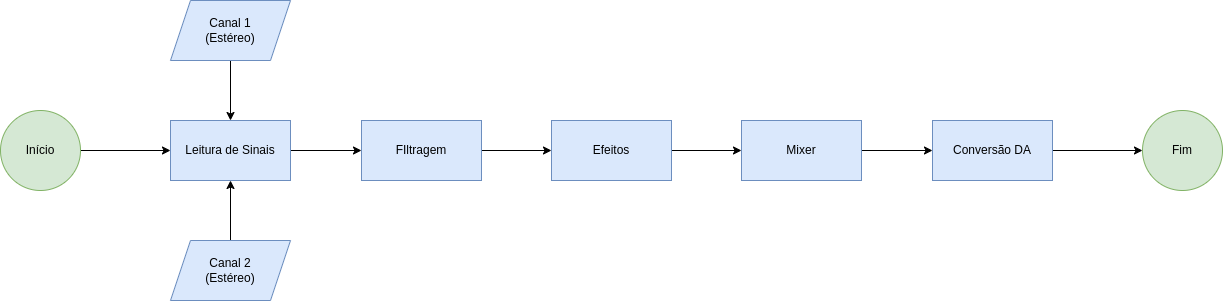
\includegraphics[width=\textwidth]{figuras/fig52.png}
    \caption{fluxograma geral do \textit{mixer}}
    \label{fig52}
\end{figure}

Os sinais provenientes de arquivos de música \textit{.wav} locais entram no sistema e são divididos em \textit{buffers}. Simultaneamente, é feita uma leitura dos valores atuais dos controles disponíveis na interface.

Com os valores dos parâmetros obtidos, a filtragem dos sinais e o processamento dos efeitos são realizados novamente para ajustar o comportamento dos sinais conforme os novos valores dos controles.

Finalmente, os sinais filtrados e os efeitos são combinados e convertidos para o formato analógico, para que possam ser reproduzidos.

Nas subseções abaixo, cada bloco presente no fluxograma geral do sistema (Figura \ref{fig52}) será detalhado em seus aspectos conceituais e processuais por meio de um subfluxograma, que descreve o processamento interno.

\subsection{Bloco de Leitura de Sinais}

Os sinais lidos incluem os sinais provenientes de arquivos digitais e os de controle provenientes de dois potenciômetros e um botão de duas posições. Os potenciômetros são utilizados para ajustar a frequência central e a quantidade de efeito desejado, enquanto o botão de duas posições é utilizado para selecionar o efeito desejado.

\begin{figure}[h]
    \centering
    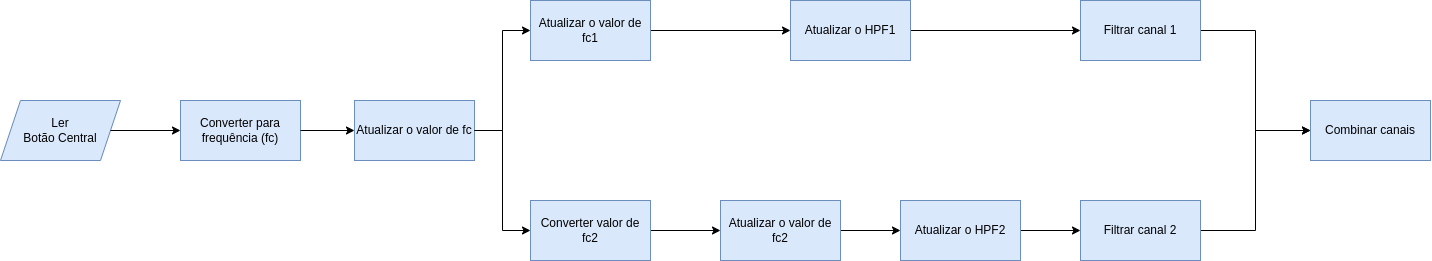
\includegraphics[width=\textwidth]{figuras/fig54.png}
    \caption{bloco de leitura de sinais}
    \label{fig54}
\end{figure}

Assim, conforme a Figura \ref{fig54}, todos os sinais analógicos de controle passarão por uma conversão analógico-digital, para que, em seguida, algumas variáveis tenham seus valores atualizados. Enquanto isso, os sinais de música obtidos de arquivos digitais já se encontram em formato digital, mas são transformados em sequência de \textit{buffers}.

\subsection{Bloco de Filtragem}

No bloco de filtragem, os sinais já estão no domínio digital. Primeiramente, deve-se ler a posição do botão central, que é obtida a partir da conversão de um sinal analógico proveniente de um potenciômetro, convertido de um sinal elétrico para um sinal digital.

Com a posição do botão, que estará em um intervalo de valores quantizados, realiza-se a normalização e conversão para um valor de frequência de corte, variando entre 20 e 22.050 Hz.

Este valor de frequência de corte é utilizado para atualizar o filtro passa-altas do canal 1, que então realiza a filtragem do sinal correspondente.

Para o canal 2, um novo valor de frequência de corte é calculado usando a expressão da Equação \ref{eq:05}. O filtro passa-altas deste canal é então ajustado conforme a nova frequência de corte, conforme ilustrado na Figura \ref{fig55}.

No bloco de filtragem, todos os sinais analógicos já estão codificados de forma que podem ser processados digitalmente. A frequência de corte central (\textit{fc}) varia entre 20 e 22.050 Hz, e os valores são atribuídos aos parâmetros \textit{fc$_{1}$} e \textit{fc$_{2}$}.

\begin{figure}[h]
    \centering
    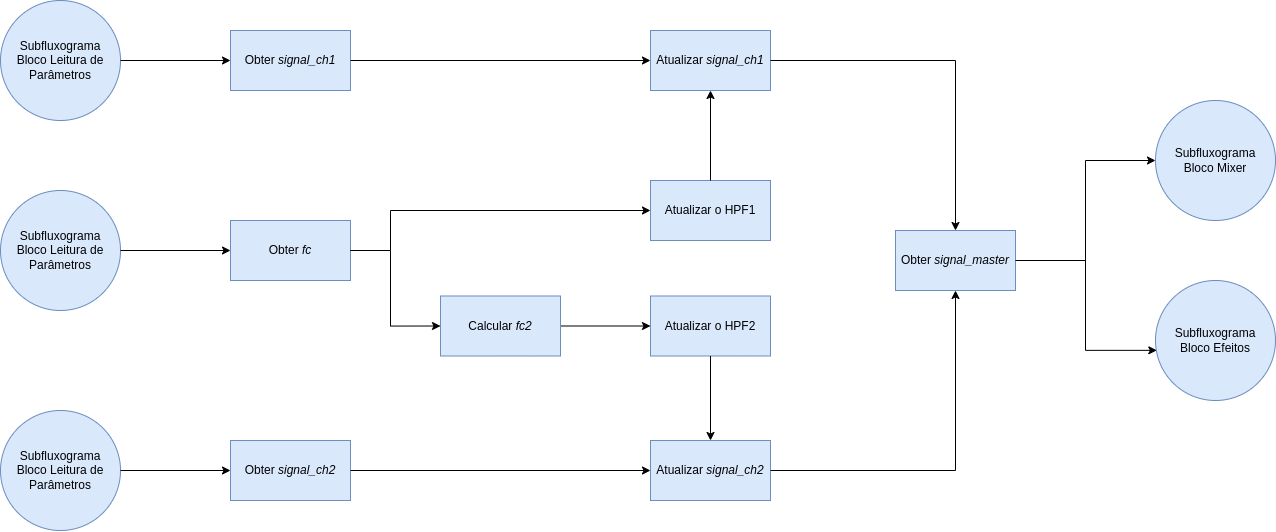
\includegraphics[width=\textwidth]{figuras/fig55.png}
    \caption{bloco de filtragem}
    \label{fig55}
\end{figure}

No subfluxograma da Figura \ref{fig55}, \textit{fc} representa a frequência de corte central, lida e convertida a partir do botão central; \textit{fc$_{1}$} é a frequência de corte para o filtro passa-altas 1 (HPF1) e \textit{fc$_{2}$} é a frequência de corte para o filtro passa-altas 2 (HPF2).

Ao final deste processo, os sinais dos dois canais são combinados, resultando no sinal \textit{signal\_master}, que é enviado ao bloco de processamento de efeitos.

\subsection{Bloco de Efeitos}

Os efeitos do \textit{mixer} podem ter seus parâmetros de reverberação e atraso configurados conforme o botão de quantidade de efeito. O parâmetro de reverberação é ajustado para 1 segundo, e o intervalo de atraso (em milissegundos) é configurado de acordo com a quantidade de efeito desejado.

\begin{figure}[h]
    \centering
    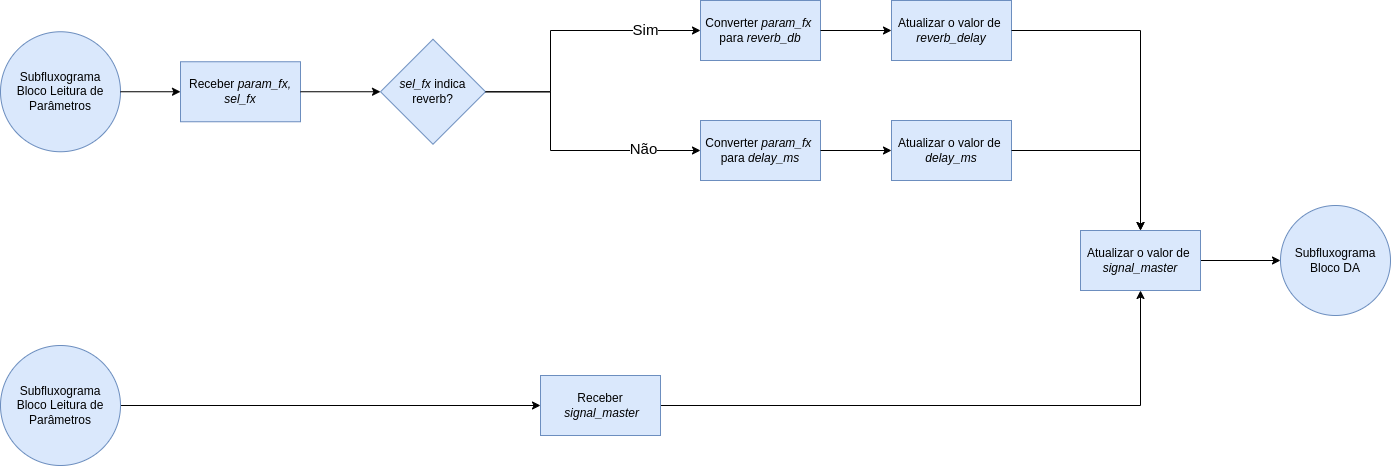
\includegraphics[width=\textwidth]{figuras/fig56.png}
    \caption{bloco de efeitos}
    \label{fig56}
\end{figure}

Além disso, o usuário pode selecionar qual efeito deseja utilizar através de um botão de duas posições, conforme ilustrado na Figura \ref{fig56}. Os parâmetros de seleção e quantidade de efeitos são obtidos do bloco de leitura de sinais. Ao final deste bloco, o sinal filtrado, já com o efeito aplicado, é atribuído ao \textit{signal\_master}.

\subsection{Bloco de Conversão DA}

O sinal de saída obtido pelo bloco \textit{Efeito} precisa ser convertido de digital para analógico para que possa ser reproduzido em um sistema de som.

\begin{figure}[h]
    \centering
    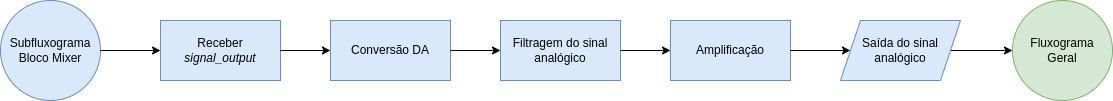
\includegraphics[width=\textwidth]{figuras/fig59.png}
    \caption{bloco de conversão digital-analógico}
    \label{fig59}
\end{figure}

Conforme mostrado na Figura \ref{fig59}, o sinal digital passará por um processo de conversão digital-analógico, para que possa ser finalmente reproduzido por caixas de som.

\newpage
\section{Prova de Conceito}

Nesta seção, é apresentada uma implementação em um ambiente virtual que simula a lógica de funcionamento do sistema.

\subsection{\textit{PureData}}

O \textit{PureData} \cite{puredata} é um ambiente de música computacional programável, projetado para análise, síntese e processamento de áudio em tempo real através de sinais digitais.

Esse ambiente permite a criação de sistemas de processamento de áudio utilizando blocos programáveis, com funções implementadas tanto pelos seus criadores quanto pela extensa comunidade de usuários.

\begin{figure}[h]
    \centering
    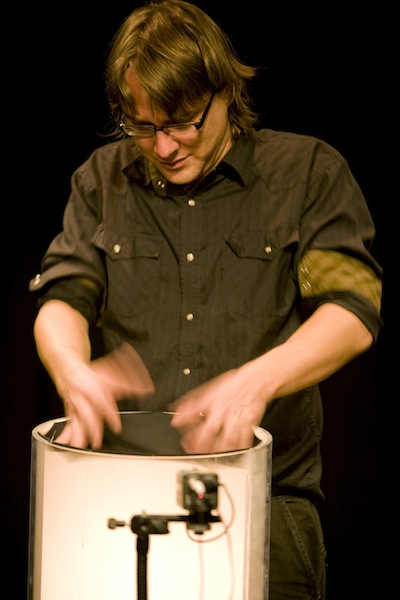
\includegraphics[width=0.3\textwidth]{figuras/fig79.jpg}
    \caption{Silent Drum de Jaime Oliver}
    \label{fig78}
\end{figure}

O \textit{PureData} contém uma extensa comunidade que desenvolve diversos tipos de projetos como instalações de arte interativas, geradores de música ambientes totalmente automatizados, uma bateria que utiliza visão computacional para controle da música, como se encontra na Figura \ref{fig78}, emuladores de equipamentos musicais, 
Outras aplicações incluem gravação, processamento e edição de áudio, \textit{samplers} e instalações de arte interativas que podem integrar sensores ou sistemas de áudio multicanal, além de projetos de projeção mapeada e muitos outros.

No \textit{PureData}, foi possível desenvolver uma prova de conceito que abrange a lógica do botão central para controle das frequências de corte, bem como o funcionamento dos efeitos. Para simular os sinais de entrada, foram utilizados arquivos \textit{.wav} locais.

A demonstração do sistema se divide em duas principais funcionalidades: filtragem e efeitos.

\subsection{Implementação de Filtragem}

A filtragem é realizada lendo dois arquivos de música no formato WAV, utilizando as funções \texttt{open}, \texttt{start} e \texttt{stop} para localizar, iniciar e parar a reprodução, respectivamente. Em seguida, o comando \texttt{readsf\textasciitilde\ 2 1e+06} é utilizado para configurar a leitura dos sinais em estéreo com um milhão de amostras no \textit{buffer}. Este processo é repetido para ambos os arquivos.

Para aplicar a filtragem, utiliza-se a função \texttt{hip\textasciitilde}, que implementa um filtro passa-altas. No entanto, o argumento da função varia entre o canal 1 e o canal 2. Como mostrado na Figura \ref{fig24}, o canal 1 ("FC do HPF1") recebe diretamente o parâmetro \textit{fc}, proveniente do \textit{slider} azul.

Por outro lado, o filtro passa-altas do canal 2 ("FC do HPF2") utiliza um valor ajustado por uma expressão anterior, conforme a Equação \ref{eq:05}. Esse ajuste assegura que uma pequena variação em \textit{fc$_{1}$} resulte em uma grande variação em \textit{fc$_{2}$}, e vice-versa. Além disso, em frequências centrais, a variação entre os canais torna-se mais semelhante. A Equação \ref{eq:05} descreve um círculo com raio igual à frequência de amostragem, com o botão centralizado no ponto (22050, 22050).

\begin{equation}  \label{eq:05}
    fc_2 = 22050 - \sqrt{22050^2 - (fc - 22050)^2}
\end{equation}

O ajuste na Equação \ref{eq:05} é projetado para ponderar mudanças nas frequências, pois mudanças lineares não são eficazes com um controle centralizado, como demonstrado pelas frequências dos canais na Figura \ref{fig45}.

\begin{figure}[h]
    \centering
    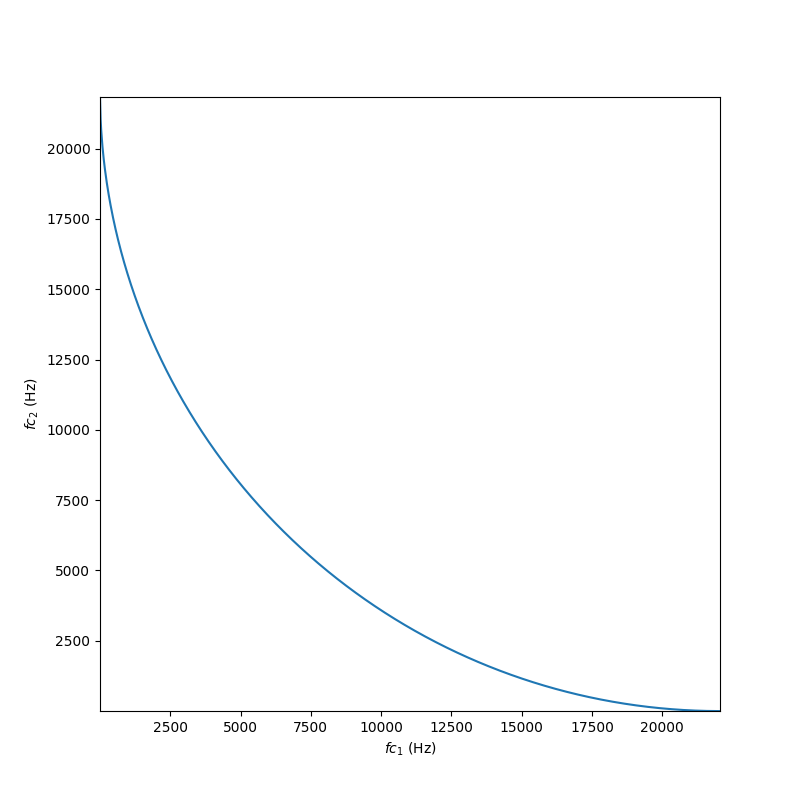
\includegraphics[width=0.7\textwidth]{figuras/fig45.png}
    \caption{expressão para a \textit{fc$_{2}$}}
    \label{fig45}
\end{figure}

Mudanças na ordem de centenas no canal 1 têm pouco impacto no canal 2, uma vez que as baixas frequências têm um ganho maior em relação às altas frequências. Essa lógica também se aplica ao outro extremo do controle de frequência.

\begin{figure}[h]
    \centering
    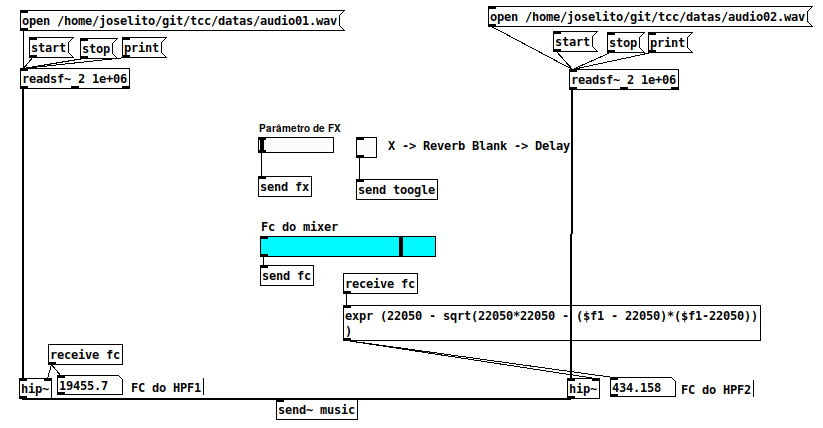
\includegraphics[width=0.9\textwidth]{figuras/fig44.png}
    \caption{lógica de funcionamento do botão central no \textit{PureData}}
    \label{fig44}
\end{figure}

Na Figura \ref{fig44}, a frequência obtida do botão central, denotada como \( f_c \), varia de 0.2 a 22050 Hz. A frequência de corte do canal 1, referida como FC do HPF1, é equivalente a \( f_c \). A frequência de corte do canal 2, identificada como FC do HPF2, é calculada pela Equação \ref{eq:05}. O sinal resultante, \texttt{send\textasciitilde\ music}, é a soma dos sinais filtrados dos canais 1 e 2.

\newpage
\subsection{Implementação de Efeitos}

A implementação dos efeitos utiliza três parâmetros principais: um botão \texttt{toggle} para alternar entre os efeitos \textit{delay} e \textit{reverb}; um \textit{slider} para ajustar parâmetros internos dos efeitos; e a frequência de corte do botão central, que automatiza o volume do efeito.

\begin{figure}[h]
    \centering
    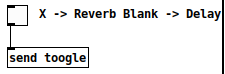
\includegraphics[width=0.3\textwidth]{figuras/fig46.png}
    \caption{botão de seleção de efeito no \textit{PureData}}
    \label{fig46}
\end{figure}

O botão \texttt{toggle} é usado para alternar entre os efeitos. Com duas posições disponíveis, sempre um efeito está ativo. Para mudar o efeito, basta alterar a posição do botão, conforme mostrado na Figura \ref{fig46}.

\begin{figure}[h]
    \centering
    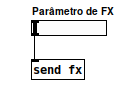
\includegraphics[width=0.2\textwidth]{figuras/fig47.png}
    \caption{botão de quantidade de efeito no \textit{PureData}}
    \label{fig47}
\end{figure}

O \textit{slider} é utilizado para ajustar os parâmetros internos de cada efeito. Seus valores variam de 0 a 1, e o botão está ilustrado na Figura \ref{fig47}.

Cada efeito utiliza o parâmetro \textit{fx} do \textit{slider} e o ajusta conforme necessário. No caso do \textit{reverb}, o valor de \textit{fx} é multiplicado por 100 para determinar a quantidade de \textit{dB} que permanece na música após 1s. Para o \textit{delay}, o valor é multiplicado por 1000, transformando-se no intervalo de tempo em \textit{ms} que o efeito permanecerá na música.

\begin{figure}[h]
    \centering
    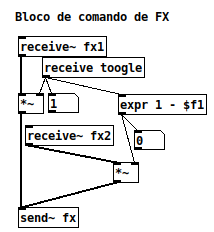
\includegraphics[width=0.3\textwidth]{figuras/fig48.png}
    \caption{lógica de seleção de efeito no \textit{PureData}}
    \label{fig48}
\end{figure}

A lógica de seleção do efeito é apresentada na Figura \ref{fig48}. Os comandos \texttt{receive\textasciitilde\ fx} inserem os efeitos como entrada. Cada volume do efeito é multiplicado pelo valor do \texttt{toggle}; um deles é multiplicado pelo valor atual enquanto o outro é multiplicado pelo inverso, permitindo que o botão \texttt{toggle} funcione como um alternador entre os efeitos.


\begin{figure}[h]
    \centering
    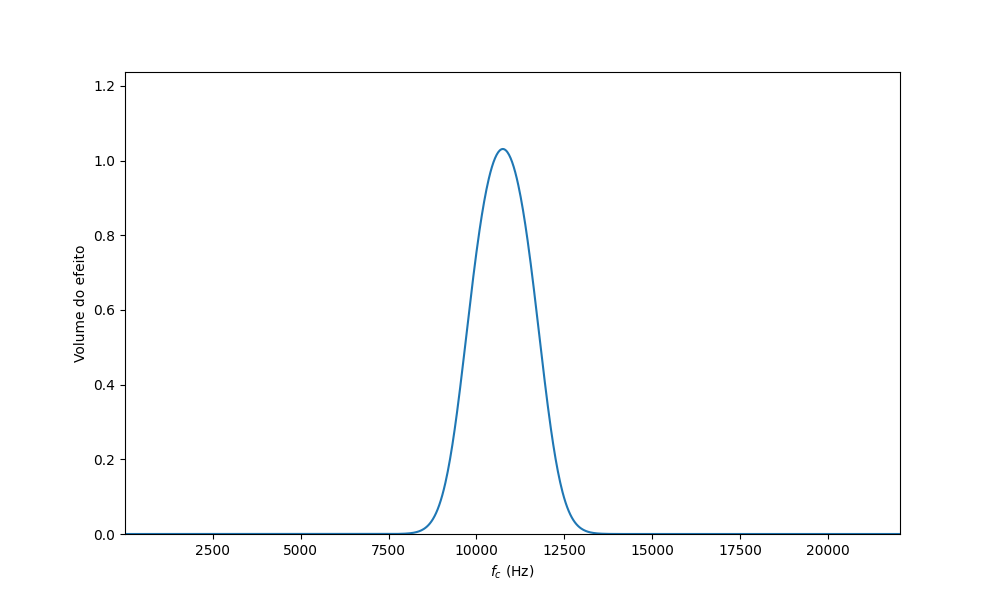
\includegraphics[width=0.9\textwidth]{figuras/fig49.png}
    \caption{variação do volume dos efeitos no \textit{PureData}}
    \label{fig49}
\end{figure}

No sistema, o volume do efeito é ajustado automaticamente com base na posição do botão central, ou seja, nas frequências de corte. A Figura \ref{fig49} ilustra a variação do volume dos efeitos em função da frequência central.

\begin{figure}[h]
    \centering
    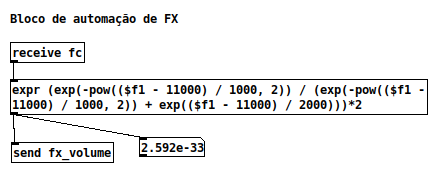
\includegraphics[width=0.6\textwidth]{figuras/fig50.png}
    \caption{implementação da variação do volume dos efeitos no \textit{PureData}}
    \label{fig50}
\end{figure}

\newpage
No \textit{PureData}, o bloco de automação do volume dos efeitos é implementado usando as operações mostradas na Figura \ref{fig50}.

\begin{figure}[h]
    \centering
    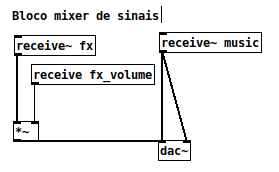
\includegraphics[width=0.3\textwidth]{figuras/fig51.png}
    \caption{soma dos sinais filtrados e dos efeitos no \textit{PureData}}
    \label{fig51}
\end{figure}

Finalmente, o sinal dos efeitos é multiplicado pelo volume dos efeitos e, em seguida, somado ao sinal filtrado, resultando no sinal de saída. Esse sinal é processado por um bloco de conversão digital-analógico e, por fim, é reproduzido. O bloco que realiza a soma dos sinais está representado na Figura \ref{fig51}.

\newpage
\section{Proposta de Implementação}

Em linhas gerais, a proposta de implementação desse projeto envolve a utilização de uma \textit{Raspberry Pi} para a escolha das músicas a serem enviadas ao \textit{mixer}, para a aquisição de sinais analógicos responsáveis pelos controles de frequência e efeitos, além de, através do conector de 3,5 mm da placa, realizar a ligação ao equipamento de sistema de som para a reprodução. 

\subsection{Implementação em Hardware}

Esta seção descreve a proposta de implementação em \textit{hardware} para o sistema de mixagem de áudio, abrangendo conectores, botões e outros componentes essenciais.

\subsubsection*{Botões}
A interação do usuário é crucial para ajustar parâmetros como frequência de corte, quantidade de efeitos e seleção do efeito desejado. Para isso, serão utilizados dois \textit{knobs} e uma chave.


\begin{figure}[h]
    \centering
    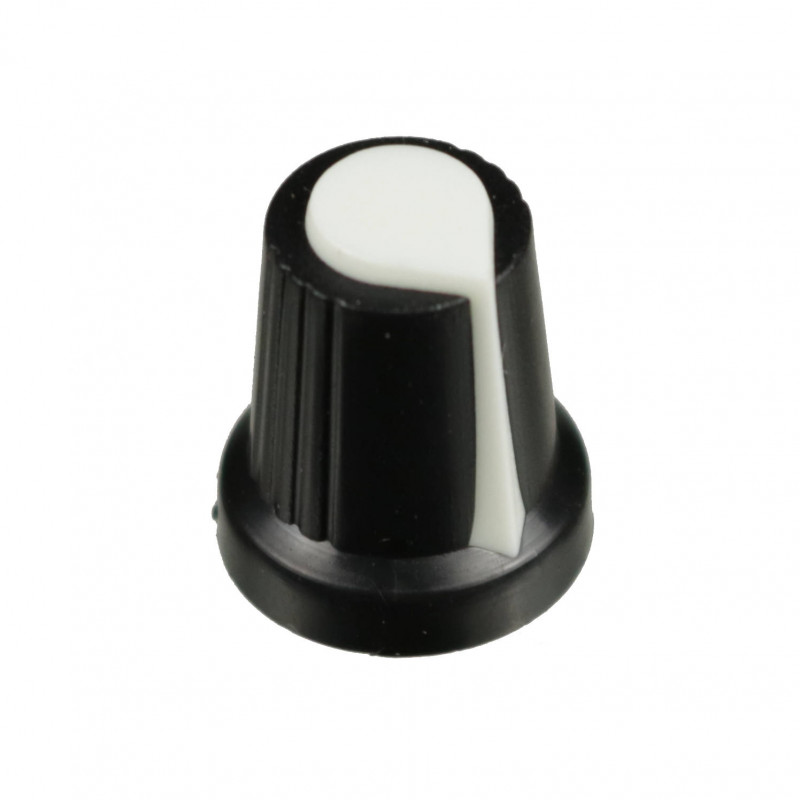
\includegraphics[width=0.3\textwidth]{figuras/fig61.jpg}
    \caption{botão \textit{knob} para frequência central e efeitos \cite{robocore}}
    \label{fig61}
\end{figure}

Os \textit{knobs} serão equipados com potenciômetros. Eles são alimentados por uma tensão, e sua posição é medida por uma tensão de saída proporcional à tensão de entrada. Essa configuração é preferida devido à precisão oferecida pelo ajuste com dois dedos, que proporciona uma mudança de frequência precisa. A Figura \ref{fig61} mostra um exemplo esperado de um \textit{knob} para ajustar a frequência central e de intensidade de efeitos.

\begin{figure}[h]
    \centering
    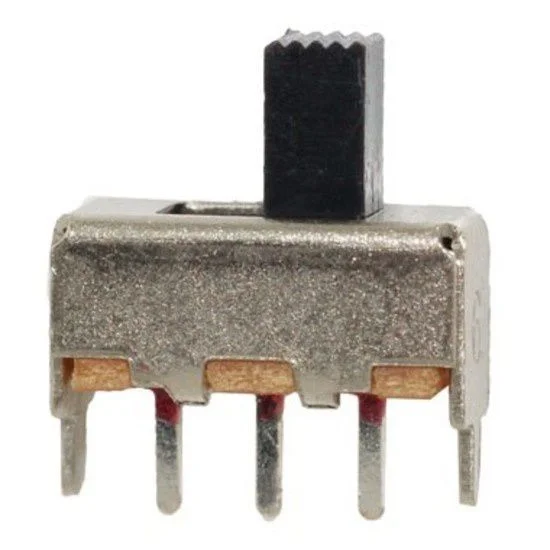
\includegraphics[width=0.3\textwidth]{figuras/fig62.png}
    \caption{botão para seleção do efeito \cite{evea}}
    \label{fig62}
\end{figure}

A chave será utilizada para selecionar entre dois efeitos distintos, gerando dois níveis de tensão: um nulo e outro de alimentação. Cada nível corresponderá a um efeito diferente. Um exemplo de botão para essa finalidade é mostrado na Figura \ref{fig62}.

Para ajustar a quantidade de efeitos desejada, será utilizado um botão semelhante ao \textit{slider}, com a mesma abordagem de controle e ajuste.

\paragraph*{Conversão AD}

A conversão analógica-digital será empregada na aquisição dos sinais de controle, ou seja, para dois potenciômetros, utilizando um conversor PCF8591, Figura \ref{fig64}, que conta com uma resolução de 8 \textit{bits}. 

\begin{figure}[h]
    \centering
    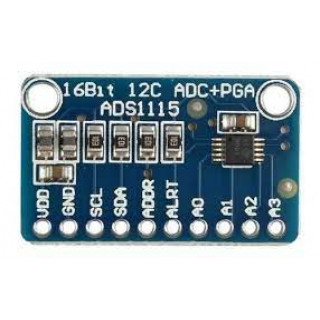
\includegraphics[width=0.5\textwidth]{figuras/fig64.jpg}
    \caption{PF8591 - conversor analógico-digital de 8 \textit{bits} \cite{saravaticomponentes}}
    \label{fig64}
\end{figure}

Para que esses sinais de controle sejam lidos, a comunicação I2C da \textit{Raspberry Pi} deve estar habilidada para a leitura.

\paragraph*{Raspberry Pi}

A unidade de processamento é o dispositivo responsável pela realização do processamento dos sinais. 

\begin{figure}[h]
    \centering
    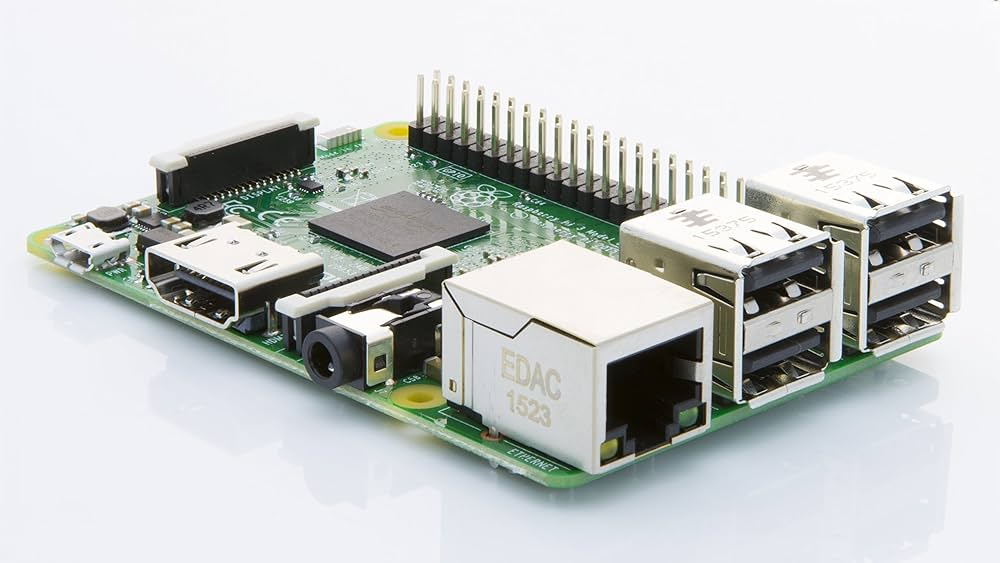
\includegraphics[width=0.5\textwidth]{figuras/fig65.jpg}
    \caption{\textit{Raspberry Pi} para processamento dos sinais \cite{adrenalineDisplaysLanar}}
    \label{fig65}
\end{figure}

Para essa tarefa, será utilizada uma \textit{Raspberry Pi}, que oferece um bom poder de processamento e flexibilidade em termos de linguagens de programação suportadas. A \textit{Raspberry Pi} é mostrada na Figura \ref{fig65}.

\paragraph*{Conversão DA}

A conversão digital-analógico é necessária para que o sinal final, após o processamento, possa ser reproduzido por sistemas de áudio que utilizam sinais analógicos. A \textit{Raspberry Pi} possui uma saída/entrada de áudio com conector de 3.5mm, conforme ilustrado na Figura \ref{fig20}.

\paragraph*{Diagrama de Conexões}

O diagrama de pinagem, Figura tal  contém o conversor AD e a \textit{Raspberry Pi 4 B}. hjjjjjjjjjjjjjjjjjjjjjjjjjjj

\begin{figure}[h]
    \centering
    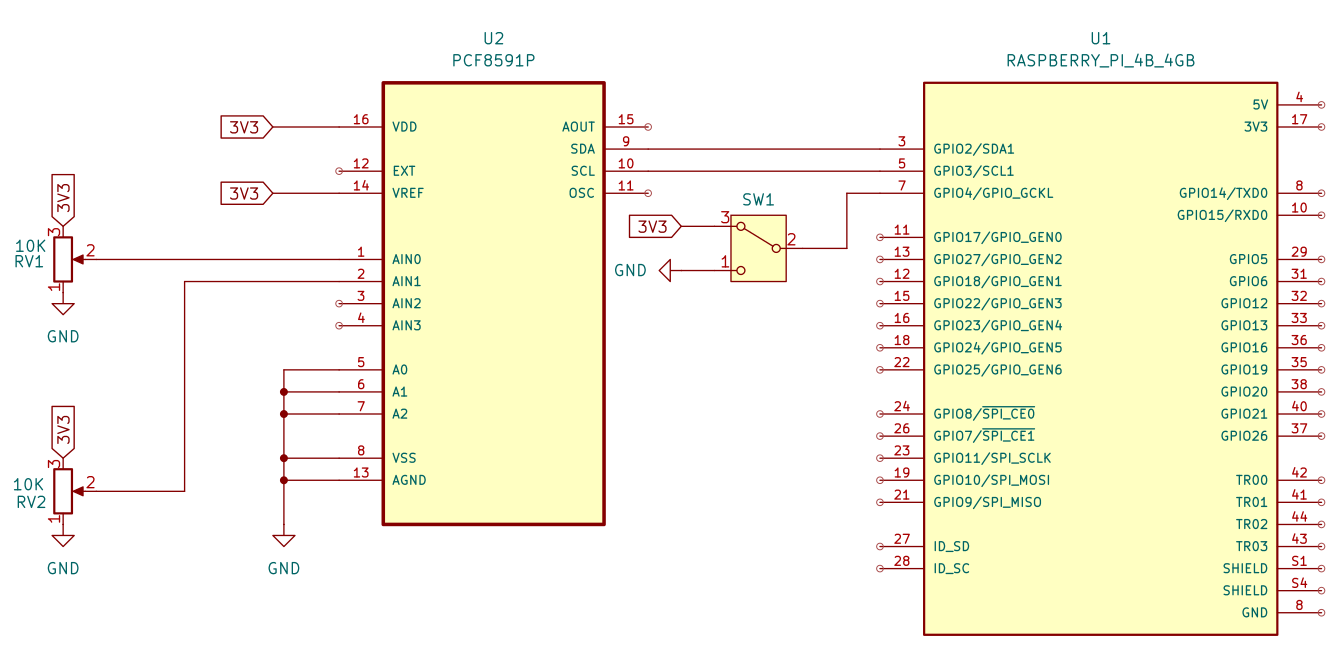
\includegraphics[width=0.5\textwidth]{figuras/fig80.png}
    \caption{Diagrama de Conexões}
    \label{fig80}
\end{figure}

\paragraph*{Lista de Materiais}
- 1 Raspberry
- 2 potenciômetros
- 1 botão hh de 2 posições
- 1 cabo 3,5 mm
- 1 cabo USB-C e USB-A
- 1 computador para acesso remoto


\subsection{Implementação em Software}

Na \textit{Raspberry Pi}, após a conversão e aquisição dos sinais, é necessário realizar o processamento para obter o sinal final. Devido à sua eficiência no processamento, a linguagem C será utilizada para a implementação do sistema.

\subsection{Protótipo de Interface de Usuário}

A interface do usuário será projetada de forma semelhante a um \textit{mixer} atual, com dois botões \textit{sliders} horizontais e um botão de duas posições. Além disso, haverá um cabo 3,5 mm para que se possa conectar a um sistema de som externo.

